%% IMPORTANT NOTICE:
%% 
%% For the copyright see the source file.
%% 
%% For distribution of the original source see the terms
%% for copying and modification in the file samples.dtx.
%% 
%% This generated file may be distributed as long as the
%% original source files, as listed above, are part of the
%% same distribution. (The sources need not necessarily be
%% in the same archive or directory.)
%%
%% The first command in your LaTeX source must be the \documentclass command.
\documentclass[sigchi]{acmart}
\usepackage{cleveref}[2012/02/15]% v0.18.4; 

%%
%% \BibTeX command to typeset BibTeX logo in the docs
\AtBeginDocument{%
  \providecommand\BibTeX{{%
    \normalfont B\kern-0.5em{\scshape i\kern-0.25em b}\kern-0.8em\TeX}}}

%% Rights management information.  This information is sent to you
%% when you complete the rights form.  These commands have SAMPLE
%% values in them; it is your responsibility as an author to replace
%% the commands and values with those provided to you when you
%% complete the rights form.
\setcopyright{acmcopyright}
\copyrightyear{2019}
\acmYear{2019}
\acmDOI{10.1145/1122445.1122456}

%% These commands are for a PROCEEDINGS abstract or paper.
\acmConference[UbiComp'19]{the ACM Conference on Ubiquitous Computing}{Sept 11--13, 2019}{London, UK}
\acmPrice{15.00}
\acmISBN{978-1-4503-9999-9/18/06}


%%
%% Submission ID.
%% Use this when submitting an article to a sponsored event. You'll
%% receive a unique submission ID from the organizers
%% of the event, and this ID should be used as the parameter to this command.
%%\acmSubmissionID{123-A56-BU3}

%%
%% end of the preamble, start of the body of the document source.
\begin{document}

%%
%% The "title" command has an optional parameter,
%% allowing the author to define a "short title" to be used in page headers.
\title{HiveTracker: Embedded 3d Positioning, Algorithms and Characterizations}
%\title{HiveTracker: Embedded 3d Positioning, Algorithms and Characterizations}

%%
%% The "author" command and its associated commands are used to define
%% the authors and their affiliations.
%% Of note is the shared affiliation of the first two authors, and the
%% "authornote" and "authornotemark" commands
%% used to denote shared contribution to the research.
\author{C\'edric Honnet}
%\orcid{1234-5678-9012}
\affiliation{%
  \institution{Sorbonne University, ISIR, CNRS}
  \streetaddress{}
  \city{Paris}
  \country{France}}
\email{cedric@honnet.eu}

\author{Gon\c{c}alo Lopes}
\affiliation{%
  \institution{NeuroGEARS Ltd}
  \streetaddress{}
  \city{London}
  \country{United Kingdom}}
\email{g.lopes@neurogears.org}

\begin{teaserfigure}
\centering
\includegraphics[width=1.0\columnwidth]{Figures/banner.jpg}
\caption{Left: the HTC Vive tracker - Right: our Hive Tracker miniaturization.}
\label{Fig:Banner}
\end{teaserfigure}

%%
%% By default, the full list of authors will be used in the page
%% headers. Often, this list is too long, and will overlap
%% other information printed in the page headers. This command allows
%% the author to define a more concise list
%% of authors' names for this purpose.
%\renewcommand{\shortauthors}{Honnet and Lopes}

%%
%% The abstract is a short summary of the work to be presented in the
%% article.
\begin{abstract}
  Recent advances in positional tracking systems for virtual and augmented reality have opened up the possibilities for ubiquitous motion capture technology in the consumer market. However, for many applications such as in performance art, athletics, neuroscience, and medicine, these systems remain too bulky and expensive for general use, and can track only a few objects at a time. In this work, we present a small wireless device that takes advantage of existing HTC Vive lighthouse tracking technology to provide affordable, scalable, and highly accurate positional tracking capabilities. This open hardware and open software project contains several elements, and the latest contributions described in this paper include: a characterization of the optical distortions of the lighthouses, a set of sensor fusion algorithms, a new cross-platform WebBLE interface, and a real-time in-browser visualization. We also introduce a new adaptive calibration using regression to estimate transformation matrices of lighthouses, and we propose an FPGA approach to allow more photodiodes, and adapt to the lighthouses V2. Finally, we show how the new developments will reduce the setup costs and increase the broader accessibility of our tracking technology.
\end{abstract}

%%
%% The code below is generated by the tool at http://dl.acm.org/ccs.cfm.
%% Please copy and paste the code instead of the example below.
%%

\begin{CCSXML}
<ccs2012>
<concept>
<concept_id>10003120.10003121.10003125</concept_id>
<concept_desc>Human-centered computing~Interaction devices</concept_desc>
<concept_significance>500</concept_significance>
</concept>
</ccs2012>
\end{CCSXML}

\ccsdesc[500]{Human-centered computing~Interaction devices}


%%
%% Keywords. The author(s) should pick words that accurately describe
%% the work being presented. Separate the keywords with commas.
\keywords{Indoor Positioning, Open-source, Low Cost, Wireless Device, Virtual Reality, 3D Tracking}


%%
%% This command processes the author and affiliation and title
%% information and builds the first part of the formatted document.
\maketitle

%%%%%%%%%%%%%%%%%%%%%%%%%%%%%%%%%%%%%%%%%%%%%%%%%%%%%%%%%%%%%%%%%%%%%%%%%%%%%%%%%%%%%%%%%%%%%%
\section{Introduction}
Robust real-time positional tracking systems have been the target of research for decades to support applications in natural user interfaces (NUI), virtual reality (VR) and augmented reality (AR). All of these interface paradigms require an accurate sampling of the spatial environment of a user, and have to be responsive in real-time in order to sustain the illusion of control. Recent developments in motion sensing and tracking technology for VR have finally moved the field of motion capture technology away from expensive custom engineered spaces with multiple cameras. The need to deploy VR at scale in the consumer market has pushed for scalable and cost-effective solutions, mostly through inside-out techniques using either computer vision based simultaneous localization and mapping (SLAM) or laser-based lighthouse approaches.

Because each device is taking care of its own localization, such inside-out solutions are inherently scalable, allowing for a much larger number of devices to coexist in the same space. This has triggered many researchers to start rethinking the entire approach to full-body motion tracking, replacing the passive reflective beads with active inside-out devices. Unfortunately, size and accuracy remain a limitation for such motion capture applications. Inside-out SLAM based computer vision devices rely on cameras and expensive processors, which both make existing controllers more bulky and increase power requirements.

\subsection{Principle}
TODO: develop / illustrate?\\\\
An alternative solution to inside-out tracking is to use a beacon-based approach, such as the one used in the HTC Vive Lighthouse tracking system. In this system, a lighthouse base station periodically sweeps the space with a laser at a fixed frequency. Photodiodes placed in tracked objects can detect these sweeps and using either information embedded in modulated light at the beam, or synchronization pulses, can reconstruct the exact angle at which the laser hit the object. Positioning information can be accurately recovered from the photodiodes as long as the timing of each laser hit can be sensed fast enough.

\subsection{Related work}
In previous work, we explored the design of a prototype called the HiveTracker \cite{Quinones2018}, that takes advantage of a rare dedicated real-time and parallel processing feature in the nRF52 microcontroller made by Nordic Semi to sense the lighthouse light sweeps without requiring a dedicated FPGA. This allowed us to design an embedded device with up to five photodiodes that is small, accurate, and cheap enough for full-body motion tracking at scale. \newline \newline
In this paper, we describe the further development of our prototype, and the main hardware and software challenges we had to overcome to increase the accessibility and ease of use of the HiveTracker beyond a proof-of-concept.

%%%%%%%%%%%%%%%%%%%%%%%%%%%%%%%%%%%%%%%%%%%%%%%%%%%%%%%%%%%%%%%%%%%%%%%%%%%%%%%%%%%%%%%%%%%%%%
\section{Contributions}

%\begin{itemize}
%  \item {\itshape Open-source firmware supporting} low-latency Bluetooth low energy (BLE) communication protocol.
%  \item {\itshape 3D reconstruction and triangulation} of positional data from each device.
%  \item {\itshape Real-time JavaScript visualization} of reconstructed positioning data for rapid-prototyping and testing.
%\end{itemize}

\subsection{Firmware}

% \begin{figure}[h]
%   \centering
%   \includegraphics[width=\linewidth]{prototype}
%   \caption{1907 Franklin Model D roadster. Photograph by Harris \&
%     Ewing, Inc. [Public domain], via Wikimedia
%     Commons. (\url{https://goo.gl/VLCRBB}).}
%   \Description{The 1907 Franklin Model D roadster.}
% \end{figure}

GitHub repository \cite{firmwareRepo}

Arduino nano 33 ble \footnote{Arduino nano 33 ble: \url{https://store.arduino.cc/usa/nano-33-ble}} 

\subsection{Optical distortion characterization}
https://hackaday.io/project/160182-hivetracker/logs

\subsection{Sensor fusion algorithms}
 (Kalman and Madgwick)
https://hackaday.io/project/160182-hivetracker/logs


\subsection{BLE interface}

The nRF52 microcontroller provides a proprietary radio communication protocol for high-bandwidth communication with a computer, but also a BLE interface. Wireless BLE communication is attractive due to its low power requirements and growing acceptance as a standard in web development stacks. In our goal to make setting up and interfacing with HiveTracker devices more accessible, we decided to embed a lightweight BLE protocol in the device firmware, allowing direct pairing from any WebBLE enabled browser.

More in the firmware \cite{firmwareRepo} and Web-App \cite{WebappRepo} repositories.

TODO: opening => cite p5.ble.js\footnote{p5.ble.js by ITP-NYU: \url{https://ItpNyu.github.io/p5ble-website/}}

\subsection{3D Reconstruction and triangulation}

For each photodiode laser hit, we can reconstruct the positioning information of the sensor relative to the origin of the base station. However, it is often desirable to position the device relative to a common reference frame. In our previous work \cite{Quinones2018}, we directly used the SteamVR calibration procedure to extract the location of each base station in absolute VR world coordinates. This was useful when integrating with existing VR applications running on the computer, for example to keep the coordinate frame of the device registered with a VR headset.

However, the base station beacons are completely passive and only require a power supply, so it would also be an advantage to allow the calibration of a common reference frame independent of SteamVR, for situations where we are running a motion capture system in full-wireless mode, independently from a computer.

To calibrate our own reference, we use a HiveTracker device as the origin, with four photodiodes arranged in a known planar configuration. For each pair of photodiode hits from the same base station, we recover two angles, from which we can reconstruct the line from the photodiode to the origin of each base station (Figure \ref{Fig:Reconstruction}A). By projecting each line onto a fixed distance plane in front of the beacon, we recover 2D positions of points at the surface of the beacon plane (Figure \ref{Fig:Reconstruction}B). Given we also know, by definition, the 3D coordinates of each of these points on the origin device, we can fully define a set of 2D/3D correspondences ($N = 4$). This is an instance of the well-known Perspective-N-Point problem for planar fiducial markers, for which there are a number of efficient solutions \cite{Lepetit2008,Garrido-Jurado2014}.

\begin{figure}[h]
\centering
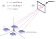
\includegraphics[width=1.0\columnwidth]{Figures/reconstruction.pdf}
\caption{Schematic of reconstruction procedure. (A): Relation of polar coordinates to cartesian coordinates, where $\theta$ and $\phi$ are the angles recovered from the device. (B): Projection of angles into fixed distance plane to generate 2D/3D correspondences.}
\label{Fig:Reconstruction}
\end{figure}

After independently computing the pose of the origin device relative to both beacons, we can make use of bundle adjustment methods such as the Levenberg-Marquardt algorithm \cite{Marquardt1963} to further improve the overall estimate of the beacon poses relative to the origin. In principle, we could extend this procedure to a grid of devices to further improve the estimated quality, as in \cite{Garrido-Jurado2014}.

\subsection{Real-time visualization}

To enable rapid-prototyping, visualization and testing of the HiveTracker performance, we developed an in-browser JavaScript interface, visualization and simulation framework using the Three.js library. This cross-platform approach allows visualizing the 3d positions in any device running Chromium or Chrome:
\\\\
TODO: add illustration and reference to repository \cite{WebappRepo}

%%%%%%%%%%%%%%%%%%%%%%%%%%%%%%%%%%%%%%%%%%%%%%%%%%%%%%%%%%%%%%%%%%%%%%%%%%%%%%%%%%%%%%%%%%%%%%
\section{Future work}

\subsection{Adaptive calibration}

TODO: Describe regression technique?\\
https://photos.app.goo.gl/VDNVeL6PZ8ZNBSpi6
\\\\
TODO: cite poser algorithms in LibSurvive? \footnote{LibSurvive: \url{https://github.com/cnlohr/libsurvive\#lists-of-components}}

\subsection{Hardware evolutions with FPGA}

%%%%%%%%%%%%%%%%%%%%%%%%%%%%%%%%%%%%%%%%%%%%%%%%%%%%%%%%%%%%%%%%%%%%%%%%%%%%%%%%%%%%%%%%%%%%%%
\section{Conclusion}

TODO

%%
%% The acknowledgments section is defined using the "acks" environment
%% (and NOT an unnumbered section). This ensures the proper
%% identification of the section in the article metadata, and the
%% consistent spelling of the heading.
\begin{acks}
The authors would like to thank Yvonne Jansen and Alexis Polti for their support and expertise offered during the developpement of this project. We would also like to thank Julien Mellet for his early work on reconstruction and fusion algorithms, Chinmay Pendharkar for introducing us to WebBLE, Olivia Seow and Chis Davis for their design and media expertise, and NeuroGEARS Ltd. for the financial support as well as the provided help. This project was partially funded by the "Human Computer Interface Prize" of the Hack-A-Day conference. Finally, this work was also partially performed within the Labex SMART (ANR-11-LABX-65), supported by French state funds managed by the ANR under reference ANR-11-IDEX-0004-02.
\end{acks}

%%
%% The next two lines define the bibliography style to be used, and
%% the bibliography file.
\bibliographystyle{ACM-Reference-Format}
\bibliography{ubicomp-2019}

%%
%% If your work has an appendix, this is the place to put it.
%\appendix

\end{document}
\endinput
%%
%% End of file `sample-sigchi.tex'.
